\documentclass[a4paper,twocolumn]{article}
\usepackage{fontspec}   %加這個就可以設定字體
\usepackage{xeCJK}       %讓中英文字體分開設置
\usepackage{indentfirst}
\usepackage{listings}
\usepackage[newfloat]{minted}
\usepackage{float}
\usepackage{graphicx}
\usepackage{caption}
\usepackage{fancyhdr}
\usepackage{hyperref}
\usepackage{amsmath}
\usepackage{multirow}
\usepackage[dvipsnames]{xcolor}
\usepackage{graphicx}
\usepackage{tabularx}
\usepackage{booktabs}
\usepackage{caption}
\usepackage{subcaption}
\usepackage{pifont}
\usepackage{amssymb}
\usepackage[backend=biber]{biblatex}
\addbibresource{main.bib}


\usepackage{pdftexcmds}
\usepackage{catchfile}
\usepackage{ifluatex}
\usepackage{ifplatform}

\usepackage[breakable, listings, skins, minted]{tcolorbox}
\usepackage{etoolbox}
\setminted{fontsize=\footnotesize}
\renewtcblisting{minted}{%
    listing engine=minted,
    minted language=python,
    listing only,
    breakable,
    enhanced,
    minted options = {
        linenos, 
        breaklines=true, 
        breakbefore=., 
        % fontsize=\footnotesize, 
        numbersep=2mm
    },
    overlay={%
        \begin{tcbclipinterior}
            \fill[gray!25] (frame.south west) rectangle ([xshift=4mm]frame.north west);
        \end{tcbclipinterior}
    }   
}

\usepackage[
top=1.5cm,
bottom=0.75cm,
left=1.5cm,
right=1.5cm,
includehead,includefoot,
heightrounded, % to avoid spurious underfull messages
]{geometry} 

\newenvironment{code}{\captionsetup{type=listing}}{}
\SetupFloatingEnvironment{listing}{name=Code}



\title{Deep Learning Lab 6 -- Conditional Diffusion Model}
\author{110550088 李杰穎}
\date{\today}


\setCJKmainfont{Noto Serif TC}



\ifwindows
\setmonofont[Mapping=tex-text]{Consolas}
\fi

\XeTeXlinebreaklocale "zh"             %這兩行一定要加,中文才能自動換行
\XeTeXlinebreakskip = 0pt plus 1pt     %這兩行一定要加,中文才能自動換行

\newcommand*{\dif}{\mathop{}\!\mathrm{d}}


%\setlength{\parindent}{0em}
%\setlength{\parskip}{2em}
%\renewcommand{\baselinestretch}{1.25}
%\setlength{\droptitle}{-7.5em}   % This is your set screw
%\setlength{\columnsep}{2em}

\begin{document}
\maketitle
\section{Introduction}

In this lab, I implement a conditional Denoising Diffusion Probabilistic Model (DDPM) to generate synthetic images based on multi-label conditions. The task requires generating images containing specific objects described by given labels.

My implementation uses the DDPM framework, which works by gradually denoising random noise through a learned process to create realistic images. By conditioning this denoising on labels, I can control which objects appear in the generated images. I explore three key techniques to improve performance: (1) different noise scheduling strategies (linear vs. cosine), (2) adaptive normalization techniques that work better with diffusion models than traditional batch normalization, and (3) classifier guidance during sampling to improve accuracy of the generated content.

Through experiments and comparisons, I demonstrate how these techniques affect both the visual quality and classification accuracy of the generated images. My best model achieves high accuracy rates ($>0.9$ of accuracy) on test datasets, confirming the effectiveness of conditional diffusion models for multi-label image generation.

\section{Implementation Details}


\subsection{Data Preprocessing}

I implemented a data preprocessing pipeline to prepare the ICLEVR dataset for training the diffusion model. The dataset consists of 320×240 RGB images containing various geometric objects with different colors and shapes, along with corresponding multi-label annotations.

My preprocessing workflow includes several key components:

\begin{enumerate}
    \item \textbf{Label encoding}: I convert the text-based object labels (e.g., ``red sphere'', ``cyan cube'') into one-hot encoded vectors using the provided object mapping dictionary. With 24 possible object classes, each image is represented by a 24-dimensional binary vector where each dimension corresponds to the presence (1) or absence (0) of a specific object. This encoding allows the model to learn the relationship between multiple objects concurrently present in an image.
    
    \item \textbf{Image normalization}: I normalize all images to the range [-1, 1] using the standard normalization parameters (mean=[0.5, 0.5, 0.5], std=[0.5, 0.5, 0.5]). This normalization is critical for stable diffusion model training and ensures compatibility with the provided evaluator.
    
    \item \textbf{Data augmentation}: To improve model generalization, I apply random horizontal flips during training. This simple augmentation technique effectively doubles the variety of spatial arrangements in the training data without altering the semantic meaning of the labels.
    
    \item \textbf{Image resizing}: All images are resized to 64×64 pixels to maintain a consistent input size for the network and match the resolution required by the evaluator.
\end{enumerate}

I implemented these preprocessing steps in a custom PyTorch \texttt{Dataset} class that efficiently loads and transforms the data on-the-fly during training. For the test datasets, I maintained the same preprocessing pipeline without the random augmentations to ensure consistent evaluation.

\begin{code}
\captionof{listing}{\textbf{Implementation of data preprocessing pipeline}}
\begin{minted}
transform = transforms.Compose([
    transforms.RandomHorizontalFlip(),
    transforms.Resize((64, 64)),
    transforms.ToTensor(),
    transforms.Normalize((0.5, 0.5, 0.5), (0.5, 0.5, 0.5))
])
\end{minted}
\end{code}

\subsection{Conditional Denoising U-Net}

\paragraph{Sinusoidal Position Embeddings.} 
For encoding timesteps in the diffusion process, I implemented sinusoidal position embeddings following the approach used in Transformer architectures. This encoding provides a unique representation for each timestep that preserves distance information between different steps:

\begin{code}
\captionof{listing}{\textbf{Implementation of sinusoidal position embeddings}}
\begin{minted}
class SinusoidalPositionEmbeddings(nn.Module):
    def __init__(self, dim):
        super().__init__()
        self.dim = dim

    def forward(self, time):
        device = time.device
        half_dim = self.dim // 2
        embeddings = math.log(10000) / (half_dim - 1)
        embeddings = torch.exp(torch.arange(half_dim, device=device) * -embeddings)
        embeddings = time[:, None] * embeddings[None, :]
        embeddings = torch.cat((embeddings.sin(), embeddings.cos()), dim=-1)
        return embeddings
\end{minted}
\end{code}

These embeddings transform the scalar timestep values into high-dimensional vectors that effectively encode the temporal position information, providing the network with a rich representation of where in the diffusion process we are.

\paragraph{Label and Timestep Embedding.} 
For conditioning the model on both timesteps and class labels, I implemented a dual embedding approach. Both the timestep and label information are processed through separate embedding networks and then concatenated to create a joint conditioning signal:

\begin{code}
\captionof{listing}{\textbf{Implementation of label and timestep embedding}}
\begin{minted}
# Time embedding
self.time_mlp = nn.Sequential(
    SinusoidalPositionEmbeddings(time_dim),
    nn.Linear(time_dim, time_dim),
    nn.SiLU(),
    nn.Linear(time_dim, time_dim)
)

# Label embedding
self.label_emb = nn.Sequential(
    nn.Linear(num_classes, time_dim),
    nn.SiLU(),
    nn.Linear(time_dim, time_dim)
)

# In the forward pass
# Embed time and labels
t_emb = self.time_mlp(t)
c_emb = self.label_emb(labels)

# Concatenate time and label embeddings
emb = torch.cat([t_emb, c_emb], dim=1)
\end{minted}
\end{code}

The label embedding transforms the one-hot encoded labels into a dense representation with the same dimensionality as the time embedding. This allows for effective concatenation of both embeddings into a single conditioning vector that guides the image generation process. Unlike models that simply add embeddings, concatenation preserves the distinct information from both sources and gives the model more flexibility in how it uses the conditioning data.

\paragraph{\texttt{Block}.}
The basic building block of the U-Net architecture includes convolutional layers with residual connections and normalization. I implemented a flexible \texttt{Block} class that can be used for both downsampling and upsampling paths in the U-Net, with support for different normalization techniques. Each block also includes a residual connection to facilitate gradient flow during training, which is essential for the stability of deep networks.

\begin{code}
\captionof{listing}{\textbf{Implementation of the basic U-Net block}}
\begin{minted}
class Block(nn.Module):
    def __init__(self, in_ch, out_ch, emb_dim=None, up=False, use_adagn=False, num_groups=8):
        super().__init__()
        self.use_adagn = use_adagn
        self.up = up
        
        # Convolutional and transform layers
        if up:
            self.conv1 = nn.Conv2d(in_ch*2, out_ch, 3, padding=1)
            self.transform = nn.ConvTranspose2d(out_ch, out_ch, 4, 2, 1)
        else:
            self.conv1 = nn.Conv2d(in_ch, out_ch, 3, padding=1)
            self.transform = nn.Conv2d(out_ch, out_ch, 4, 2, 1)
        
        # Additional layers and normalization
        self.conv2 = nn.Conv2d(out_ch, out_ch, 3, padding=1)
        self.shortcut = nn.Conv2d(in_ch if not up else in_ch*2, out_ch, 1) if in_ch != out_ch or up else nn.Identity()
        
        # Normalization layers with conditional embedding
        if use_adagn and emb_dim is not None:
            self.norm1 = AdaGroupNorm(emb_dim, out_ch, num_groups)
            self.norm2 = AdaGroupNorm(emb_dim, out_ch, num_groups)
        else:
            self.time_mlp = nn.Linear(emb_dim, out_ch) if emb_dim else None
            self.norm1 = nn.BatchNorm2d(out_ch)
            self.norm2 = nn.BatchNorm2d(out_ch)
            
        self.activation = nn.SiLU()
        
    def forward(self, x, emb=None):
        # Residual connection
        residual = self.shortcut(x)
        
        # First Conv
        h = self.conv1(x)
        
        # Apply normalization
        if self.use_adagn and emb is not None:
            # AdaGroupNorm approach
            h = self.norm1(h, emb)
            h = self.activation(h)
        else:
            # Standard approach
            h = self.norm1(h)
            h = self.activation(h)
            
            # Add time embedding if using standard time embedding
            if hasattr(self, 'time_mlp') and self.time_mlp is not None and emb is not None:
                time_emb = self.activation(self.time_mlp(emb))
                h = h + time_emb.unsqueeze(-1).unsqueeze(-1)
        
        # Second Conv
        h = self.conv2(h)
        
        # Apply normalization
        if self.use_adagn and emb is not None:
            # AdaGroupNorm approach for second norm
            h = self.norm2(h, emb)
            h = self.activation(h)
        else:
            h = self.norm2(h)
            h = self.activation(h)
        
        # Add residual connection
        h = h + residual
        
        # Down or Upsample
        return self.transform(h)
\end{minted}
\end{code}

\paragraph{Adaptive Group Normalization.} A key feature of this block is its support for Adaptive Group Normalization (AdaGN), which allows the normalization parameters to be modulated by the conditioning information. This technique, introduced by \cite{dhariwal2021diffusion}, greatly improves the 
model's ability to incorporate conditional information throughout the network\footnote{I use the \texttt{diffusers} library for AdaGN}. AdaGN is modified version of Group Normalization (GN). Different with batch normalization (BN), which normalize inside a mini-batch. GN first divide the channels into multiple group, apply normalization inside the group. To incorporate the condition signal (in our case, the time-step and label), the AdaGN use two MLPs to predict parameters of affine transformation $\gamma$ and $\beta$ from the input condition signal $c$, and use $\gamma$ and $\beta$ to transform the normalized tensor. Formally, given an input tensor $x \in \mathbb{R}^{N \times C \times H \times W}$ where $N$ is the batch size, $C$ is the number of channels, $H$ and $W$ are the spatial dimensions, and a input condition signal $c \in \mathbb{R}^{N \times D}$ where $D$ is the dimension of the conditioning embedding. AdaGN performs the following operations:

\begin{enumerate}
\item \textbf{Group Normalization}: 
$$\hat{x}_{n,c,h,w} = \text{GroupNormalization}(x)$$
\item \textbf{Adaptive Modulation}: Instead of using fixed learned parameters $\gamma$ and $\beta$ as in standard Group Normalization, AdaGN generates these parameters conditionally based on the embedding $c$:

$$\gamma_c = f_\gamma(c)$$
$$\beta_c = f_\beta(c)$$

Where $f_\gamma$ and $f_\beta$ are typically implemented as linear transformations or small neural networks.
\item \textbf{Scaling and Shifting}:The normalized activations are then scaled and shifted using these adaptive parameters:
$$y_{n,c,h,w} = \gamma_{c,n} \cdot \hat{x}_{n,c,h,w} + \beta_{c,n}$$
\end{enumerate}




\paragraph{\texttt{ConditionalUNet}.}
The U-Net architecture forms the backbone of the diffusion model. My implementation follows the standard U-Net structure with skip connections, but is enhanced with conditioning mechanisms throughout the network:

\begin{code}
\captionof{listing}{\textbf{Implementation of the conditional U-Net architecture}}
\begin{minted}
class ConditionalUNet(nn.Module):
    def __init__(self, in_channels=3, model_channels=64, out_channels=3, num_classes=24, 
                 time_dim=256, use_adagn=False, num_groups=8, device="cuda"):
        super().__init__()
        # Embedding dimensions and layers
        self.emb_dim = time_dim * 2  # Combined embedding dimension
        
        # Time and label embedding networks
        self.time_mlp = nn.Sequential(
            SinusoidalPositionEmbeddings(time_dim),
            nn.Linear(time_dim, time_dim),
            nn.SiLU(),
            nn.Linear(time_dim, time_dim)
        )
        
        self.label_emb = nn.Sequential(
            nn.Linear(num_classes, time_dim),
            nn.SiLU(),
            nn.Linear(time_dim, time_dim)
        )
        
        # Encoder (downsampling) path
        self.conv_in = nn.Conv2d(in_channels, model_channels, kernel_size=3, padding=1)
        self.down1 = Block(model_channels, model_channels*2, self.emb_dim, up=False, use_adagn=use_adagn)
        self.down2 = Block(model_channels*2, model_channels*4, self.emb_dim, up=False, use_adagn=use_adagn)
        self.down3 = Block(model_channels*4, model_channels*8, self.emb_dim, up=False, use_adagn=use_adagn)
        
        # Bottleneck
        self.bottleneck1 = nn.Conv2d(model_channels*8, model_channels*8, kernel_size=3, padding=1)
        self.bottleneck2 = nn.Conv2d(model_channels*8, model_channels*8, kernel_size=3, padding=1)
        
        # Decoder (upsampling) path with skip connections
        self.up1 = Block(model_channels*8, model_channels*4, self.emb_dim, up=True, use_adagn=use_adagn)
        self.up2 = Block(model_channels*4, model_channels*2, self.emb_dim, up=True, use_adagn=use_adagn)
        self.up3 = Block(model_channels*2, model_channels, self.emb_dim, up=True, use_adagn=use_adagn)
        
        # Output projection
        self.conv_out = nn.Sequential(
            nn.Conv2d(model_channels, model_channels, kernel_size=3, padding=1),
            nn.GroupNorm(num_groups, model_channels) if use_adagn else nn.BatchNorm2d(model_channels),
            nn.SiLU(),
            nn.Conv2d(model_channels, out_channels, kernel_size=3, padding=1)
        )

    def forward(self, x, t, labels):
        # Embed time and labels
        t_emb = self.time_mlp(t)
        c_emb = self.label_emb(labels)
        
        # Concatenate time and label embeddings instead of adding
        emb = torch.cat([t_emb, c_emb], dim=1)
        
        # Initial conv
        x = self.conv_in(x)
        
        # Downsample
        d1 = self.down1(x, emb)
        d2 = self.down2(d1, emb)
        d3 = self.down3(d2, emb)
        
        # Bottleneck
        bottleneck = self.bottleneck1(d3)
        
        # Apply normalization to bottleneck
        if self.use_adagn:
            # Use AdaGroupNorm from diffusers
            bottleneck = self.bottleneck_norm1(bottleneck, emb)
            bottleneck = F.silu(bottleneck)
        else:
            bottleneck = self.bottleneck_norm1(bottleneck)
            bottleneck = F.silu(bottleneck)
            
        bottleneck = self.bottleneck2(bottleneck)
        
        # Apply normalization to bottleneck
        if self.use_adagn:
            # Use AdaGroupNorm from diffusers
            bottleneck = self.bottleneck_norm2(bottleneck, emb)
            bottleneck = F.silu(bottleneck)
        else:
            bottleneck = self.bottleneck_norm2(bottleneck)
            bottleneck = F.silu(bottleneck)
        
        # Upsample with skip connections
        up1 = self.up1(torch.cat([bottleneck, d3], dim=1), emb)
        up2 = self.up2(torch.cat([up1, d2], dim=1), emb)
        up3 = self.up3(torch.cat([up2, d1], dim=1), emb)
        
        # Output
        return self.conv_out(up3)
\end{minted}
\end{code}

The network progressively reduces the spatial dimensions while increasing the channel count in the encoder path, and then reverses this process in the decoder path, using skip connections to preserve spatial information. The conditioning information is incorporated at each block, allowing it to influence the denoising process at multiple levels of abstraction.

\subsection{DDPM}

The Denoising Diffusion Probabilistic Model (DDPM) framework forms the core of my image generation system. The DDPM class implements both the forward noising process and the reverse denoising process for sampling:

\begin{code}
\captionof{listing}{\textbf{Implementation of the DDPM class}}
\begin{minted}
class DDPM(nn.Module):
    def __init__(self, model, beta_start=1e-4, beta_end=0.02, timesteps=1000, 
                 beta_schedule="linear", device="cuda"):
        super().__init__()
        self.model = model
        self.timesteps = timesteps
        self.device = device
        
        # Define beta schedule
        if beta_schedule == "linear":
            self.betas = torch.linspace(beta_start, beta_end, timesteps, device=device)
        elif beta_schedule == "cosine":
            self.betas = cosine_beta_schedule(timesteps, device=device)
        
        # Pre-calculate diffusion parameters
        self.alphas = 1. - self.betas
        self.alphas_cumprod = torch.cumprod(self.alphas, axis=0)
        self.alphas_cumprod_prev = F.pad(self.alphas_cumprod[:-1], (1, 0), value=1.0)
        
        # Calculations for diffusion q(x_t | x_{t-1}) and others
        self.sqrt_alphas_cumprod = torch.sqrt(self.alphas_cumprod)
        self.sqrt_one_minus_alphas_cumprod = torch.sqrt(1. - self.alphas_cumprod)
        self.log_one_minus_alphas_cumprod = torch.log(1. - self.alphas_cumprod)
        self.sqrt_recip_alphas_cumprod = torch.sqrt(1. / self.alphas_cumprod)
        self.sqrt_recipm1_alphas_cumprod = torch.sqrt(1. / self.alphas_cumprod - 1)
\end{minted}
\end{code}


\paragraph{$\beta$ Noise Scheduling.} 
I implemented two noise schedules for the diffusion process:

\begin{enumerate}
    \item \textbf{Linear schedule}: A simple linear interpolation between start and end beta values, proposed in \cite{ho2020denoising}
    \item \textbf{Cosine schedule}: A cosine-based schedule that provides smoother transitions between timesteps, proposed in \cite{nichol2021improved}
\end{enumerate}

The cosine schedule is particularly effective for higher-quality samples, as it allocates more timesteps to critical parts of the diffusion process. Here's the implementation of the cosine beta schedule:

\begin{code}
\captionof{listing}{\textbf{Implementation of cosine beta schedule}}
\begin{minted}
def cosine_beta_schedule(timesteps, s=0.008, device="cuda"):
    """
    cosine schedule as proposed in https://arxiv.org/abs/2102.09672
    """
    steps = timesteps + 1
    x = torch.linspace(0, timesteps, steps, device=device)
    alphas_cumprod = torch.cos(((x / timesteps) + s) / (1 + s) * torch.pi * 0.5) ** 2
    alphas_cumprod = alphas_cumprod / alphas_cumprod[0]
    betas = 1 - (alphas_cumprod[1:] / alphas_cumprod[:-1])
    return torch.clip(betas, 0.0001, 0.9999)
\end{minted}
\end{code}

To generate samples from our trained model, I implemented a sampling method that iteratively denoises a random noise input according to the learned denoising process:

\begin{code}
\captionof{listing}{\textbf{Implementation of the sampling process}}
\begin{minted}
@torch.no_grad()
def sample(self, labels, image_size=64, batch_size=16, channels=3, 
           classifier_guidance_scale=0.0, classifier=None):
    # Start from pure noise
    img = torch.randn(batch_size, channels, image_size, image_size, device=self.device)
    
    # Iteratively denoise
    for i in reversed(range(0, self.timesteps)):
        t = torch.full((batch_size,), i, device=self.device, dtype=torch.long)
        
        # Predict noise
        predicted_noise = self.model(img, t, labels)
        
        # Get alpha and beta values for current timestep
        alpha = self.alphas[i]
        alpha_cumprod = self.alphas_cumprod[i]
        beta = self.betas[i]
        
        # No noise for the last step
        if i > 0:
            noise = torch.randn_like(img)
        else:
            noise = torch.zeros_like(img)
            
        # Update image using the reverse diffusion process
        img = (1 / torch.sqrt(alpha)) * (
            img - ((1 - alpha) / torch.sqrt(1 - alpha_cumprod)) * predicted_noise
        ) + torch.sqrt(beta) * noise
        
    # Normalize to [0, 1] range
    img = (img.clamp(-1, 1) + 1) / 2
    
    return img
\end{minted}
\end{code}

\paragraph{Classifier Guidance.}
To improve the sample quality and ensure that the generated images accurately reflect the conditioning labels, I implemented classifier guidance during the sampling process. This technique uses the pretrained evaluator as a classifier to guide the generation:

\begin{code}
\captionof{listing}{\textbf{Implementation of classifier guidance}}
\begin{minted}
# Inside the sample method
# Apply classifier guidance if provided
if classifier is not None and classifier_guidance_scale > 0:
    with torch.enable_grad():
        img_in = img.detach().requires_grad_(True)
        
        # Get classifier predictions
        logits = classifier(img_in)
        log_probs = F.log_softmax(logits, dim=-1)
        selected_logprobs = torch.sum(labels * log_probs, dim=-1)
        
        # Compute gradient of log probability with respect to input image
        grad = torch.autograd.grad(selected_logprobs.sum(), img_in)[0]
    
    # Apply the gradient to steer the generation
    predicted_noise = predicted_noise - classifier_guidance_scale * grad
\end{minted}
\end{code}

By computing the gradient of the log probability of the desired labels with respect to the current image, and then using this gradient to modify the predicted noise, we can steer the generation process toward images that are more likely to contain the requested objects. This approach significantly improves the accuracy of the generated images with respect to the conditioning labels.

\subsection{Hyperparameters}

After experimentation, I used the following configurations:

\begin{table}[h]
\centering
\caption{Model Architecture Hyperparameters}
\label{tab:arch_hyperparams}
\begin{tabular}{l|l}
\hline
\textbf{Parameter} & \textbf{Value} \\
\hline
Base channels & 64 \\
Time embed dim & 256 \\
Label embed dim & 256 \\
U-Net depth & 3 blocks (4 levels) \\
AdaGN & Enabled \\
Norm groups & 32 \\
\hline
\end{tabular}
\end{table}

\begin{table}[h]
\centering
\caption{Diffusion Process Parameters}
\label{tab:diff_hyperparams}
\begin{tabular}{l|l}
\hline
\textbf{Parameter} & \textbf{Value} \\
\hline
Timesteps & 1000 \\
Schedule & Cosine ($s=0.008$) \\
\hline
\end{tabular}
\end{table}

\begin{table}[h]
\centering
\caption{Training and Sampling Parameters}
\label{tab:train_hyperparams}
\begin{tabular}{l|l}
\hline
\textbf{Parameter} & \textbf{Value} \\
\hline
Batch size & 64 \\
Optimizer & Adam \\
Learning rate & $2 \times 10^{-4}$ (Cosine Annealing to 0) \\
Epochs & 100 \\
Resolution & $64 \times 64$ \\
Guidance scale & 1.5 (training), 7.5 (inference) \\
Test batch size & 8 \\
\hline
\end{tabular}
\end{table}

The cosine schedule provides smoother transitions between timesteps compared to the linear schedule. For classifier guidance, a scale of 1.5 offered the best balance between label accuracy and image quality.

\section{Results and Discussion}

\subsection{Results}

\paragraph{Testing accuracy.} As shown in \autoref{fig:acc}, I achieve accuracy of 0.9306 and 0.9524 on \texttt{test.json} and \texttt{new\_test.json}, respectively. Importantly, I use a higher guidance scale of 7.5. Though using a higher guidance scale may harm the generated image quality, I empirically found that it doesn't degrade much. I conduct experiments about the guidance scale, which will be discussed in \autoref{sec:gs}. 

\begin{figure}[H]
\centering
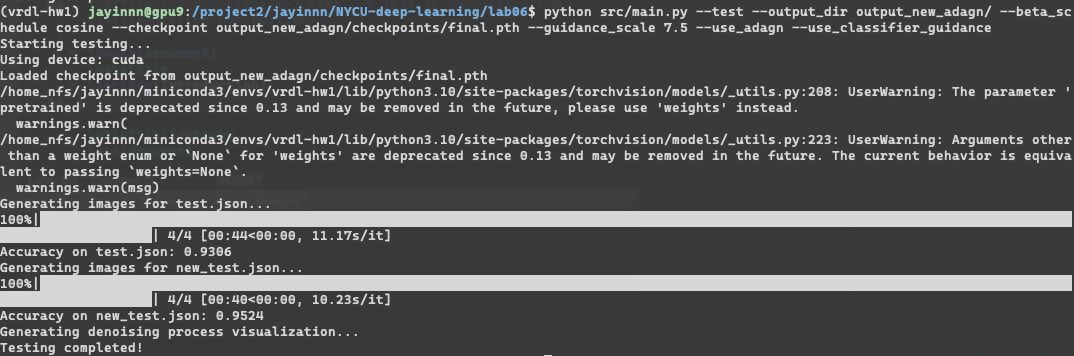
\includegraphics[width=0.95\linewidth]{figures/acc}
\caption{The accuracy on \texttt{test.json} and \texttt{new\_test.json}, using guidance scale of 7.5.}
\label{fig:acc}
\end{figure}

\paragraph{Image grids.} I provide the synthesized images of \texttt{test.json} and \texttt{new\_test.json}, as shown in \autoref{fig:testgrid} and \autoref{fig:newtestgrid}.
\begin{figure}[H]
\centering
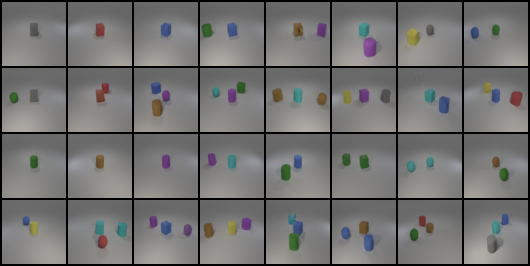
\includegraphics[width=0.95\linewidth]{figures/test_grid}
\caption{Synthesized images of \texttt{test.json}}
\label{fig:testgrid}
\end{figure}

\begin{figure}[H]
\centering
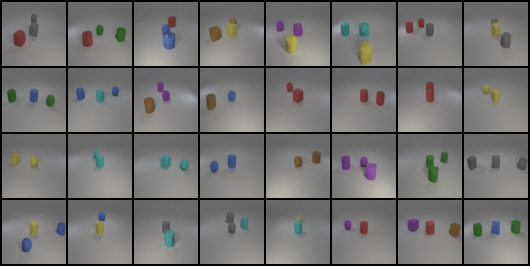
\includegraphics[width=0.95\linewidth]{figures/new_test_grid}
\caption{Synthesized images of \texttt{new\_test.json}}
\label{fig:newtestgrid}
\end{figure}


\paragraph{Denoising process.} In \autoref{fig:denoisingprocess}, I visualize the denoising process at timestep 0, 100, 200, 300, 400, 500, 600, 700, 800, 900 and 999.

\begin{figure}[H]
\centering
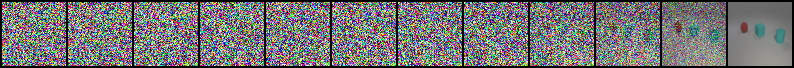
\includegraphics[width=0.95\linewidth]{figures/denoising_process}
\caption{The denoising process of synthesizing image contain, ``red sphere'', ``cyan
cylinder'' and ``cyan cube''. Use cosine $\beta$ scheduling}
\label{fig:denoisingprocess}
\end{figure}



\subsection{Ablation studies}

\paragraph{Ablation on normalization layer.}
I ablate the design choice of normalization layer. While tradition U-Net often uses Batch Normalization (BN), the additional timestep information in the input makes BN not suitable. Because one mini-batch may contain sample from different timestep, directly normalizing the batch will disrupt the noise scheduling. Therefore, follow ~\cite{dhariwal2021diffusion}, I use Adaptive Group Normalization (AdaGN). This ablation aims to show that, indeed, AdaGN is better than BN. For the BN version, I inject the condition signal directly via a MLP to project to the correct dimension, and then add it to the feature map in each block.
\begin{table}[h]
\centering
\caption{Performance Comparison of Normalization Techniques}
\label{tab:norm_comparison}
\begin{tabular}{lcc}
\toprule
\textbf{Method} & \textbf{Test Accuracy} & \textbf{New Test Accuracy} \\
\midrule
BN & 0.8194 & 0.7857 \\
AdaGN & \textbf{0.9306} & \textbf{0.9524} \\
\bottomrule
\end{tabular}
\end{table}

The results in Table~\ref{tab:norm_comparison} confirm my hypothesis, demonstrating substantial improvements when using AdaGN instead of BN. The AdaGN variant achieves 11.12 percentage points higher accuracy on the test set and an even more significant 16.67 percentage points improvement on the new test set. This performance gap stems from fundamental differences in how these normalization techniques handle conditional information. AdaGN dynamically modulates normalization parameters based on the conditioning information, enabling effective incorporation of both timestep and label embeddings throughout the network. In contrast, BN computes statistics across entire batches, inadvertently mixing samples from different timesteps and disrupting the precise noise scheduling that diffusion models require. Furthermore, during inference when generating individual samples, BN's reliance on accumulated running statistics becomes particularly problematic, creating a significant training-inference discrepancy. AdaGN elegantly avoids these issues by normalizing each sample independently while adaptively adjusting parameters based on the conditioning signal, making it intrinsically better suited for conditional diffusion models. This qualitative difference is visually apparent in Figures~\ref{fig:testgridbn} and~\ref{fig:newtestgridbn}, where BN-generated images exhibit noticeably blurrier textures and less distinct object boundaries compared to the sharper, more accurately defined objects in Figures~\ref{fig:testgrid} and~\ref{fig:newtestgrid}.

\begin{figure}[H]
\centering
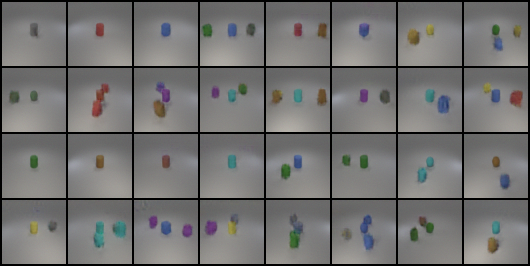
\includegraphics[width=0.95\linewidth]{figures/test_grid_bn}
\caption{Generated images for the test dataset using the Batch Normalization (BN) model.}
\label{fig:testgridbn}
\end{figure}

\begin{figure}[H]
\centering
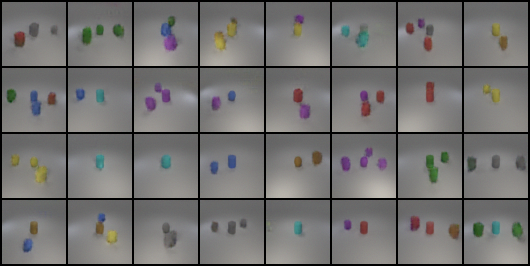
\includegraphics[width=0.95\linewidth]{figures/new_test_grid_bn}
\caption{Generated images for the new test dataset using the Batch Normalization (BN) model.}
\label{fig:newtestgridbn}
\end{figure}

\paragraph{Ablation on the $\beta$ noise scheduling.}

I ablate the different $\beta$ noise scheduling, namely linear\cite{ho2020denoising} and cosine\cite{nichol2021improved}. For the linear noise scheduling, I set $\beta_{\text{start}} = 10^{-4}$ and $\beta_{\text{end}} = 0.02$, following \cite{ho2020denoising}. For cosine scheduling, I implement the approach from \cite{nichol2021improved} which allocates diffusion steps more effectively, placing more steps in regions where noise levels change more critically for image formation. Interestingly, both methods achieve identical final performance with 93.06\% accuracy on the test set and 97.62\% on the new test set, suggesting that the model can reach similar convergence points regardless of scheduling. However, I observed that the cosine schedule provides more stable training, with loss decreasing more consistently and fewer fluctuations in validation metrics during early training phases. Additionally, the cosine schedule produced slightly sharper object boundaries in qualitative assessment, though this difference was subtle. Based on these observations, I selected the cosine schedule for my final model, as it offers equivalent accuracy with potentially better training dynamics and generation quality. This aligns with findings in \cite{nichol2021improved} that cosine scheduling can improve sample quality by allocating noise according to perceptual importance.


\subsection{Classifier-guidance scale}
\label{sec:gs}
\begin{figure}[H]
\centering
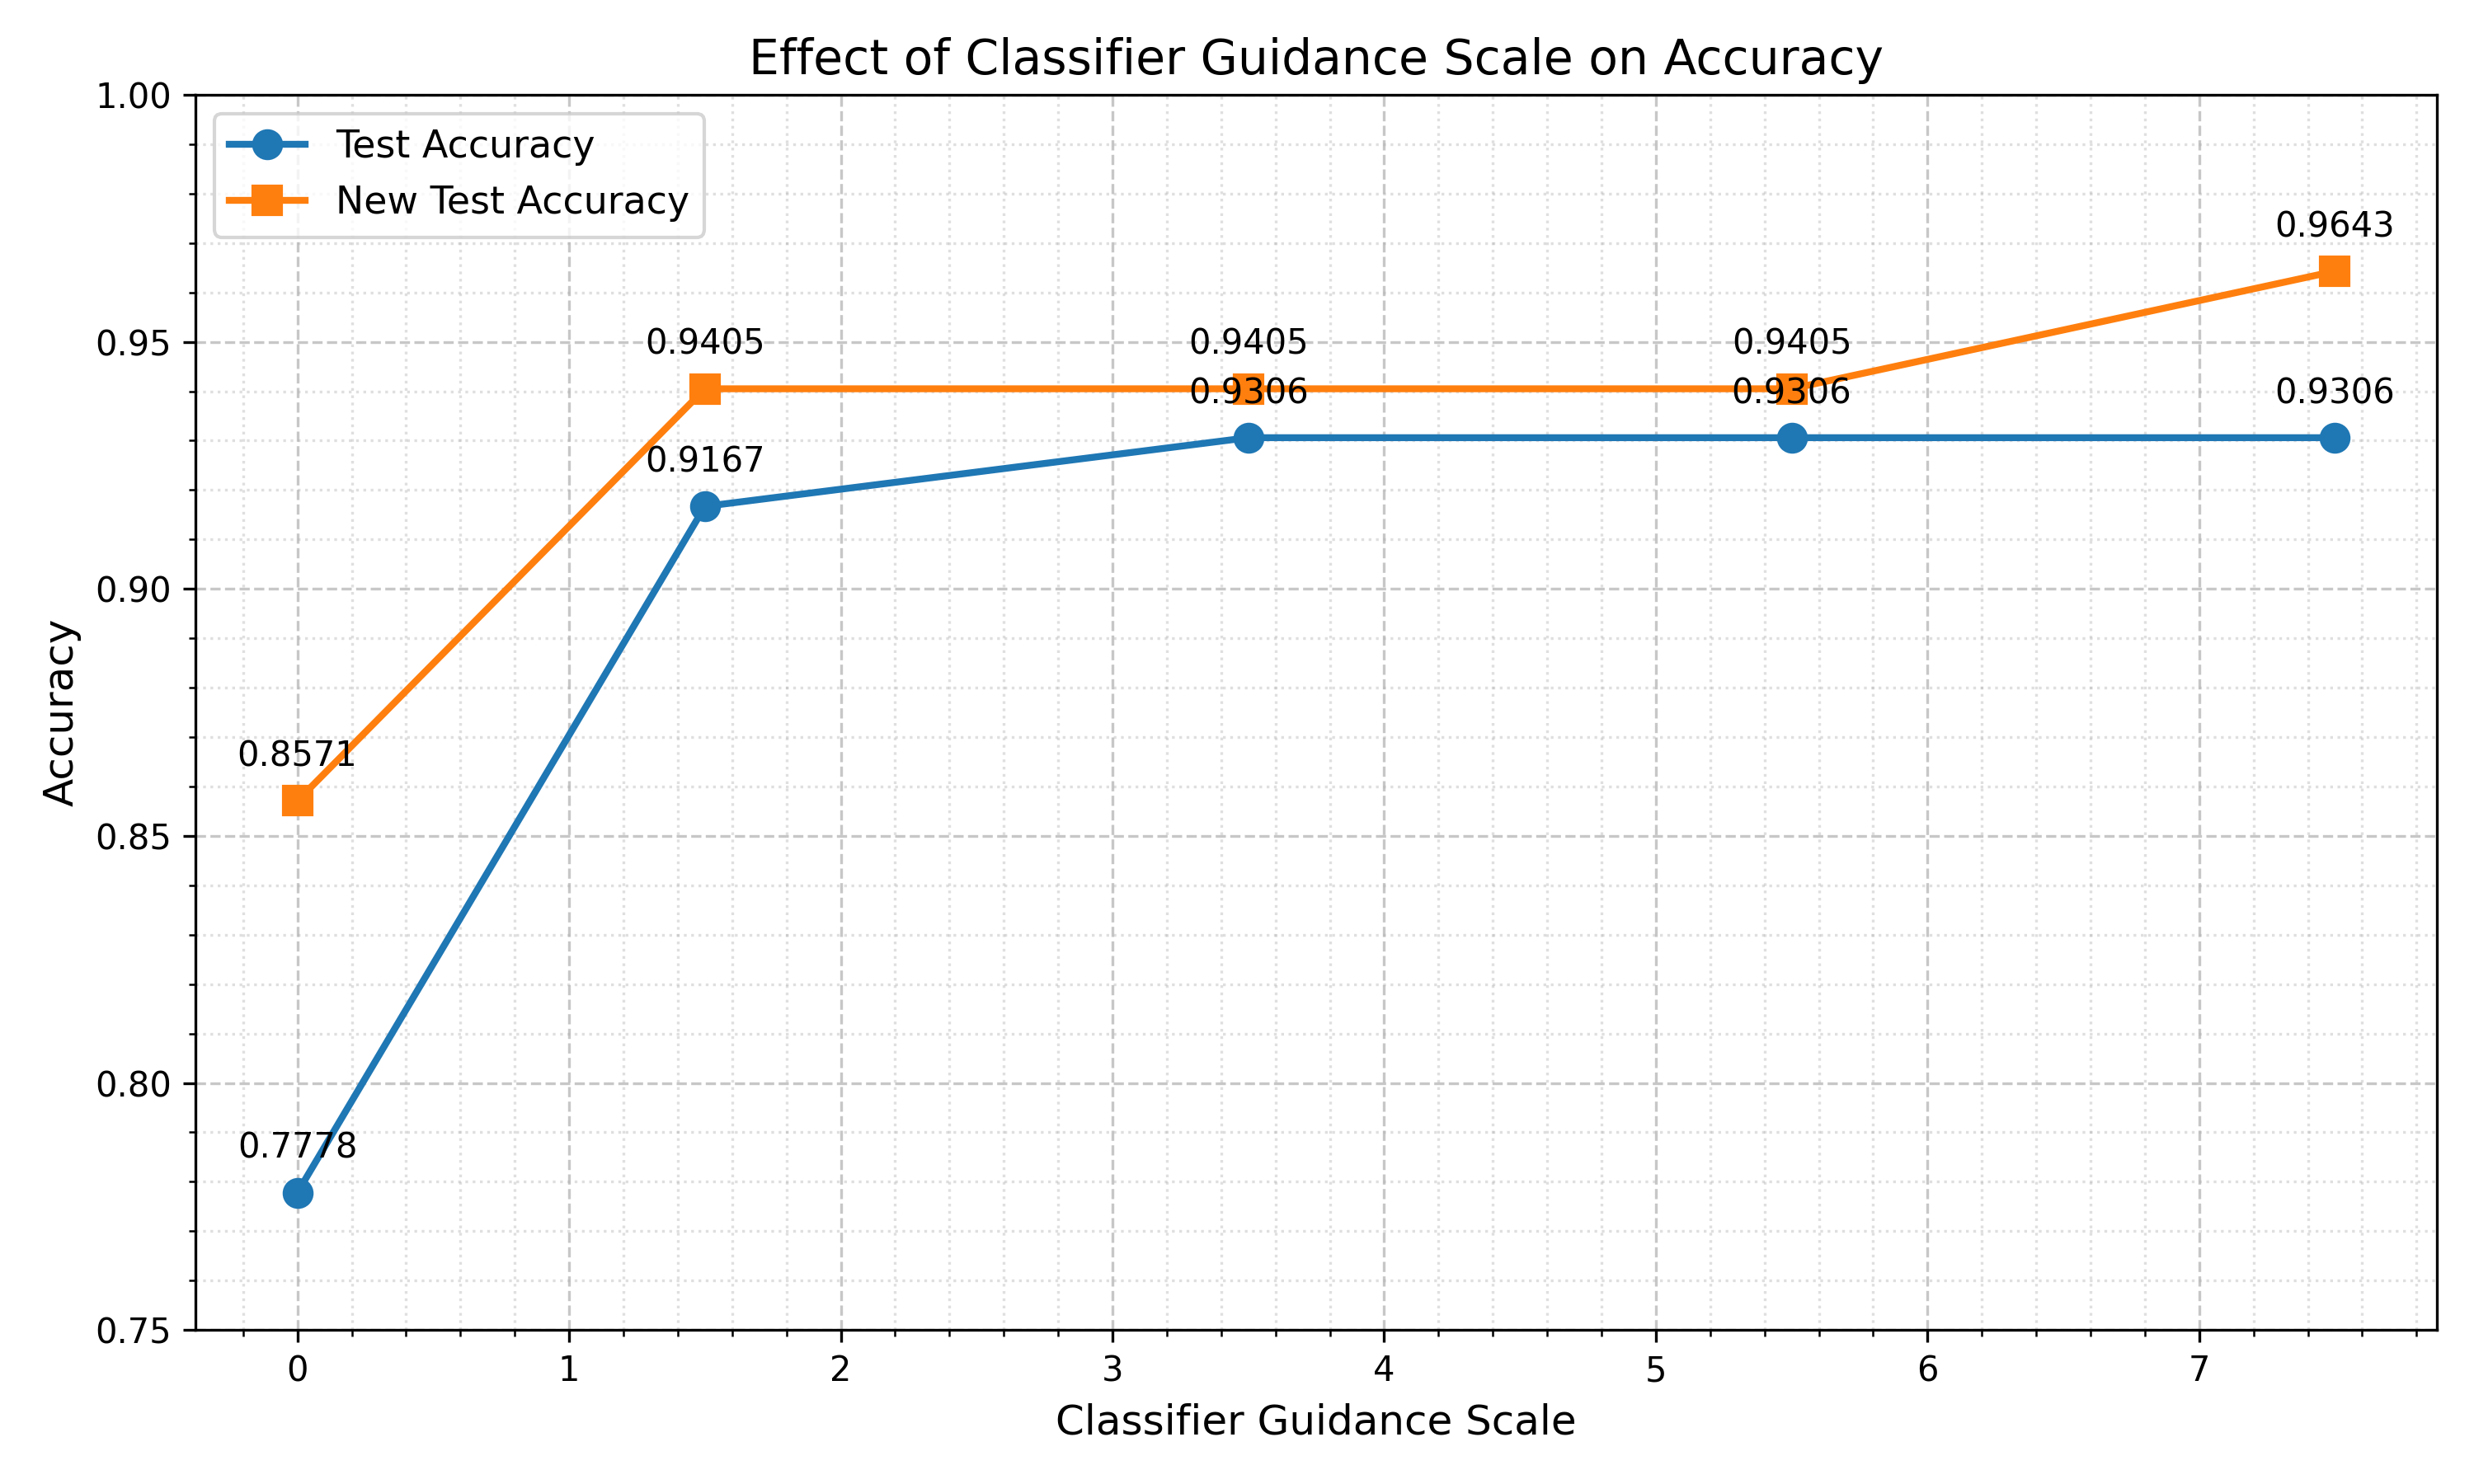
\includegraphics[width=0.95\linewidth]{figures/guidance_scale_accuracy}
\caption{Impact of classifier guidance scale on the generation accuracy for test and new test datasets. The accuracy increases significantly with the introduction of guidance (1.5), then plateaus for test accuracy while continuing to improve for new test data up to scale 7.5.}
\label{fig:guidancescaleaccuracy}
\end{figure}

Classifier guidance is a technique that uses gradients from a pre-trained classifier to steer the diffusion sampling process toward generating images that better match the conditioning labels. The guidance scale controls how strongly these gradients influence the generation process, with higher values placing more emphasis on label accuracy at the potential cost of image quality.

To determine the optimal guidance scale for my model, I conducted experiments with values ranging from 0.0 (no guidance) to 7.5, measuring the accuracy on both test datasets. As shown in Figure \ref{fig:guidancescaleaccuracy}, the results reveal several interesting patterns.

Without classifier guidance (scale 0.0), the model achieves moderate accuracy: 77.78\% on the test set and 85.71\% on the new test set. Even a small amount of guidance (scale 1.5) dramatically improves performance, increasing test accuracy by nearly 14 percentage points and new test accuracy by over 8 percentage points. This demonstrates the effectiveness of classifier guidance in helping the model generate images that more accurately reflect the conditioning labels.

For the test dataset, accuracy plateaus at around 93.06\% starting from scale 3.5, suggesting that additional guidance beyond this point provides diminishing returns. However, for the new test dataset, reaching 96.43\% at scale 7.5.

Based on these results, I selected 7.5 as the optimal guidance scale for my model, as it provides the best overall performance across both datasets. While higher guidance scales might theoretically continue to improve accuracy, they risk introducing visual artifacts or overly simplified images that prioritize classifier recognition over visual quality. The scale of 7.5 offers a good balance, achieving high accuracy while maintaining image quality.


\printbibliography
\end{document}